\documentclass{article}
\usepackage{graphicx} % Required for inserting images
\usepackage[%  
    colorlinks=true,
    pdfborder={0 0 0},
    linkcolor=red
]{hyperref}
\usepackage{geometry}
 \geometry{
 a4paper,
 total={173mm, 247mm},
 left=18mm,
 top=20mm,
 }

\title{Brew Bucks}
\author{Nimesh Garg, Peidong Liu, Lars Moan, Daniel Morgan, Manav Trivedi, Sai Karthikeya Vermulapalli}
\date{April 27, 2024}

\begin{document}

\maketitle
\pagebreak

\tableofcontents
\pagebreak

\section{Abstract}
The original proposal can be found \href{https://csse6400.github.io/project-proposal-2024/s4780791/proposal.html}{here}.

\section{Changes}
Describe and justify any changes made to the project from what was outlined in the proposal.

\subsubsection*{1. Add Simplicity Quality Attribute}
There are items below that correspond to features under the functionality section in the original proposal. The items indicate why simplicity is relevant to the application.

\medskip \begin{minipage}{\dimexpr\textwidth-0.25cm}
0. Seamless coffee ordering experience
\begin{itemize}
    \item General goal for Brewbucks application
    \item Deliver essential functionality for smooth user experience
\end{itemize}

1. Extensive Coffee Menu 
\begin{itemize}
    \item Desire for customers to explore a range of foods with ease
    \item A user-friendly interface for the menu is recognised
    \item Categorised browsing for 'easy' navigation through menu items
\end{itemize}

3. Easy Payments
\begin{itemize}
    \item Feature is regarded as something that is easy to perform or in other words, simple
\end{itemize}
\end{minipage}

\bigskip \noindent The features above reflect the need for simplicity in the application. However, there currently isn't a quality attribute to bring this to the forefront of a developer's attention. Consequently, it is likely to be overlooked through the project's implementation. The team decided to approach this problem by establishing simplicity as a quality attribute. Ideally, this will encourage simple solutions to problems encountered when developing Brewbucks, just as the author implies. This goes for the architecture, features and UI. This feels justified given the proposal's author has emphasised the need for customers to engage with the platform with ease. Therefore, simplicity can be regarded as an obvious, yet neglected quality attribute. 

\subsubsection*{2. Removal of Customizable Ordering}
\begin{itemize}
    \item Simplifies user interface and architecture
    \item Eliminates complications with orders including adjusting espresso shot strength and selecting dairy-free alternatives
    \item Eliminates the need for a separate database dedicated to posted customizable orders
    \item Eliminates the need for a separate user interface dedicated to uploaded customizable orders
    \item Eliminates the need for ingredient configurations on drinks (breakdown of ingredients for drinks would likely result in another database)
\end{itemize}

\bigskip \noindent This feature is considered by the team to be secondary. The purpose of Brewbucks is to create 'a smooth and hassle-free coffee ordering experience'. Brewbuck's appeal is 'Queue-Free Coffee Ordering at Your Fingertips' as noted in the proposal's title. Therefore, Brewbucks intends to eliminate queues, by facilitating online ordering and payments. Naturally, the user would have a quick and smooth experience if they know when their coffee is ready for collection. This is why the order tracking feature has also been prioritised. Based on the goal statement for Brewbucks, customizable ordering does not appear to be essential to delivering the app's benefits. The rewards from omitting this feature can also be seen in the architecture. The effects described above reflect the simplifications from removing customizable ordering. Bear in mind, simplicity is now an important quality attribute for the application. Aside from this, separating the database would detract from the benefits of a shared database, i.e., data consistency and integrity promotes reliability. Consequently, feature would make more sense in a long term iteration of the application. 

\subsubsection*{3. Removal of Reward Point System}
\begin{itemize}
    \item Simplifies payments system by eliminating need for discounting
    \item Simplifies user experience - adding a feature such as reward points would mean having to explain it to customers, this introduces the need for additional pages
    \item Simplifies user interfaces - an additional user interface would potentially be added to enable customers to view their accumulated points
    \item Remove the need for additional logic such as reward floors and ceilings, reward constraints
    \item Removes additional table from shared database
\end{itemize}

\bigskip \noindent This feature is also considered secondary by the team. A customer will turn to Brewbucks for online ordering, payments and tracking. A reward point system and loyalty program are common in brick-and-mortar cafes. What this means is that, a customer will not likely expect Brewbucks to have such a feature. The appeal for Brewbucks, to reiterate, is to create'a smooth and hassle-free coffee ordering experience'. Consequently, this feature was not regarded as essential for implementation. The team felt it more important to dedicate the time saved into implementing a system that does well to satisfy the quality attributes. This feature, did not directly contribute to any quality attributes, nor is it an architecturally significant requirement. There are also the benefits gained by simplifying the user experience, see them listed above. This is an important quality attribute to be preserved. A rushed implementation of this feature could emerge as a reliability or security flaw.

\section{Architecture Options}
What architectural design patterns were considered and their pros and cons.

\subsection{Event-Driven Architecture}
\subsubsection*{Pros for System Functionality}
\begin{itemize}
    \item Asynchronous communication can help with taking orders and processing payments concurrently
    \item Event handler cohesion principle can be used to scale for high load tasks, such as taking orders and processing payments
    \item Broker topology is suitable for sequential events, e.g., take coffee order, handle payment, make coffee, finish order
\end{itemize}
\subsubsection*{Cons for System Functionality}
\begin{itemize}
    \item Asynchronous communication and the inevitable communication failures add to architecture complexity
\end{itemize}

\subsubsection*{Pros for ASRs}
\begin{itemize}
    \item Broker topology is simple to implement and optimised for performance, responsiveness, scalability, extensibility, fault tolerance and low coupling
    \item Event handlers can be scaled to better manage their load through a load balancer and automated scaling mechanism
    \item Libraries and cloud-computing platforms make it easier to implement underlying functionality of event broker
    \item Have a channel implement a queue for scalability
\end{itemize}
\subsubsection*{Cons for ASRs}
\begin{itemize}
    \item It can be a challenge to implement event handlers so that they don't rely on event broker's deployment structure.
    \item Testing and debugging is hard with asynchronous communication
    \item When recoverability is compromised, implementing the broker topology is hard (bad for availability)
    \item Development team unfamiliar with supporting libraries and services
    \item Implementing event-driven architecture is complex
\end{itemize}

\subsection{Microservices Architecture}
\subsubsection*{Pros for System Functionality}
\begin{itemize}
    \item Application is suited to independently deployable, loosely coupled, components, e.g., a service for orders, payment, tracking
    \item Can distribute operations asynchronously using a message broker - helps with taking orders and processing payments concurrently
\end{itemize}   
\subsubsection*{Cons for System Functionality}
\begin{itemize}
    \item Operations may need to be implemented with complex, non-ACID transaction management (loose coupling requires services to have independent databases)
    \item Risk of tight design-time coupling between services, which means time consuming lockstep changes
    \item Design challenges with implementing distributed operations
\end{itemize}

\subsubsection*{Pros for ASRs}
\begin{itemize}
    \item Services can consist of a small number of subdomains - makes for greater simplicity, understanding and maintainability
    \item Different services can use different technology stacks and can be upgraded independently (extensibility)
    \item Subdomains can be split by concerns for separate services - supports scalability, availability, security etc
\end{itemize}
\subsubsection*{Cons for ASRs}
\begin{itemize}
    \item Maintainability affected by complex distributed operations, making troubleshooting trickier
    \item Availability affected by distributed operations with tight runtime coupling between services
    \item Implementing a microservices architecture is complex
\end{itemize}

\subsection{Brewbucks Architecture Justification}
\subsubsection*{Pros for System Functionality}
\begin{itemize}
    \item Shared database offers data integrity and consistency. It's needed for reliable order tracking, history
    \item Food Purchasing service can manage all database transactions for placing an order, e.g., when a food is no longer available, the service can rollback the transaction to guarantee data integrity (supports reliability)
\end{itemize}
\subsubsection*{Cons for System Functionality and ASRs}
\begin{itemize}
    \item Cons (and justification for these) are discussed in section 5 Trade-offs 
\end{itemize}

\subsubsection*{Pros for ASRs}
\begin{itemize}
    \item Simple, flexible, distributed architecture
    \item Domain partitioning offers high-level modularity 
    \item Domain distribution supports multiple instances of a service using a load balancer, enabling greater availability and some scalability 
    \item Service design locator pattern used to provide easier extensibility
    \item Stateless service pattern for multiple running instances of a service offers greater reliability
    \item All services can use the same façade design pattern for simplicity
    \item Support for the independent service principle makes for a simple, maintainable, deployable and modular design
\end{itemize}

\medskip \noindent \textbf{Simplicity QA}
\hfill \break Remember that simplicity is a newly introduced quality attribute. To achieve this, the principle of KISS was followed when developing Brewbucks. This idea applies especially when approaching the architecture for the project. To meet the desired quality attributes, a simple solution can be adopted with slight enhancements. As it stands, the event-driven and microservices architecture do not pursue a simple solution. A complex solution also becomes less feasible when the project's time constraints are considered. More to this, the development team felt that microservices would introduce complications associated with implementing distributed operations and tight design-time coupling between services. While event-driven would bring challenges in trying to successfully implement the event and worker queues.

\medskip \noindent \textbf{Well Satisfied QAs}
\hfill \break Service based architecture does well to meet several quality attributes. This includes: availability, reliability, extensibility, testability and deployability. Testability has been given higher priority for this project as evaluation is a key part of the delivery. Note that event-driven architecture falls short here as there are complications in testing and debugging asynchronous communication. Meanwhile, microservices introduces some complexity when trying to understand the call chain for any given request. Several microservices would not be easy to understand, hindering the application's maintainability and testing. Service-based architectures limits the number of network calls as it groups largers chunks of code together by domain (will boost performance) (Fletcher, 2016).

\medskip \noindent \textbf{Partially Satisfied QAs}
\hfill \break Conversely, there are quality attributes only partially met: interoperability, security and scalability. Scalability levels are considered sufficient for coffee orders. In a one hour period, it's expected that the app will receive 100 - 115 orders (Coffee School, 2022). See the testing evaluation for a summary of how the app performed under such conditions. Interoperability can be achieved with the API abstraction principle. Additional security support can be added by using an API layer to add security policies.

\hfill \break For these reasons, the team felt that the service-based architecture balances functionality, quality attributes and project constraints quite well.  

\section{Architecture}
Brewbucks software architecture description.

\begin{figure}
    \centering
    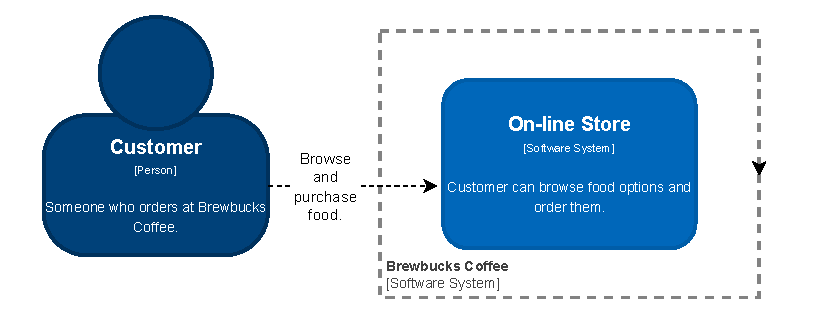
\includegraphics[width=0.5\linewidth]{model//c4//pdf/context_drawio.pdf}
    \caption{Context Diagram}
    \label{fig:context}
\end{figure}

\subsubsection*{General Overview of Architecture}
\medskip \noindent Application has a service-based architecture
\begin{itemize}
    \item Five distributable services based on app's core functionality (see figure \ref{fig:container})
    \begin{itemize}
     \item Supports features such as viewing menu items, payments, order history and status
     \item Easily extensible for new features
     \item Domain partitioning offers high-level modularity and deployability
     \item Enables multiple instances of a service using a load balancer for greater availability and some scalability
   \end{itemize}
   \item Service APIs implemented for interoperability support
   \item Shared database for all containers 
    \begin{itemize}
     \item Supports reliability by ensuring data integrity and consistency
    \end{itemize}
   \item Services don't retain any state from previous calls - stateless service pattern
    \begin{itemize}
    \item Offers higher reliability, in terms of running multiple instances of a service
    \item  Request calls are designed so that information on whose details are asked for, are provided. Calls are /users/\{userid\}/orders/\{orderid\}/items as opposed to /items.
     \item Example? Food Purchasing service is responsible for finalising an order by accepting payment. Say there are 10 instances for Food Purchasing service, it doesn't matter which instance serves the request, customer always gets same data. Consequently, instances can scale up and down as needed.
     \item Handle traffic for Brewbucks application with load balancer
    \end{itemize}
    \item Check the status of instances with a healthcheck through AWS EC2 (maintainability and testing support)
    \item Service-based principles encourage a simple, maintainable, deployable and modular design
    \begin{itemize}
     \item Independent service principle is followed whereby none of the services depends on another
    \end{itemize}
\end{itemize}

\subsubsection*{Key Observations \ref{fig:container}} 
\begin{itemize}
    \item The single database server with logical partitioning of the data satisfies the system in terms of performance. Examples of partitioning include the payments and order table
    \item A separate user interface was implemented for employee accounts to change a customer's order status
    \item Domain services are not used by external systems, so a reverse proxy was not necessary. Payment service has a simple implementation as opposed to using an external payment provider 
\end{itemize}

\subsubsection*{Design Problem Consideration}
\bigskip \hfill \begin{minipage}{\dimexpr\textwidth-0.5cm}
\textbf{1. Shared database complications:} More services makes the database design more complicated. Performance bottlenecks may occur. 

\medskip \textbf{Solution?} User interface will not be complicated as there are only five services. Database design was relatively simple given this app can be treated as a small-sized system. It's expected that coffee orders are 100 - 115 in a 1 hour busy period. See 7 Evaluation for more.
\end{minipage}

\newgeometry{left=1.5cm,bottom=2.0cm,right=1.5cm,top=2.0cm}
\begin{figure}
    \centering
    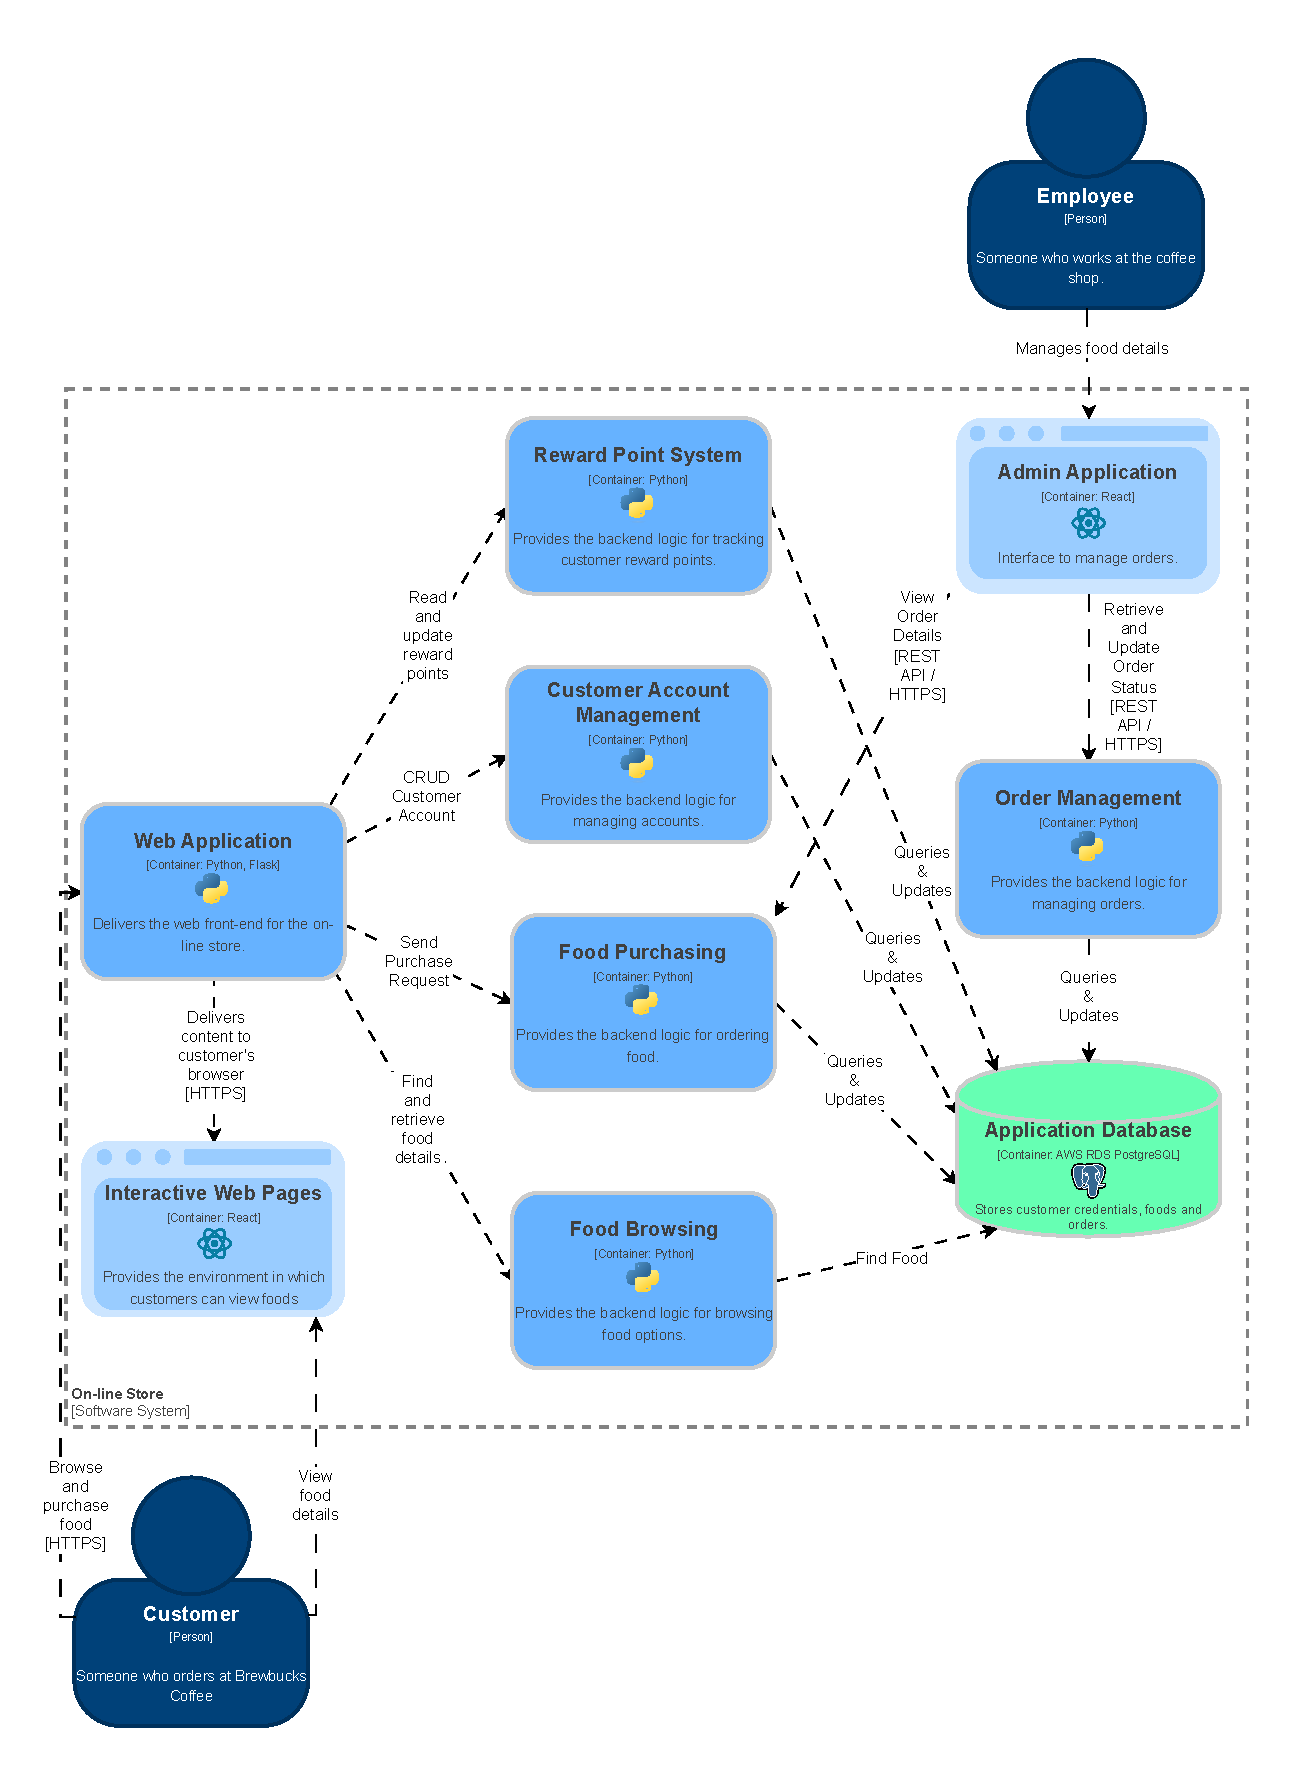
\includegraphics[width=0.80\linewidth]{model//c4//pdf/on-line-store-container-diagram_drawio.pdf}
    \caption{Container Diagram}
    \label{fig:container}
\end{figure}
\begin{figure}
    \centering
    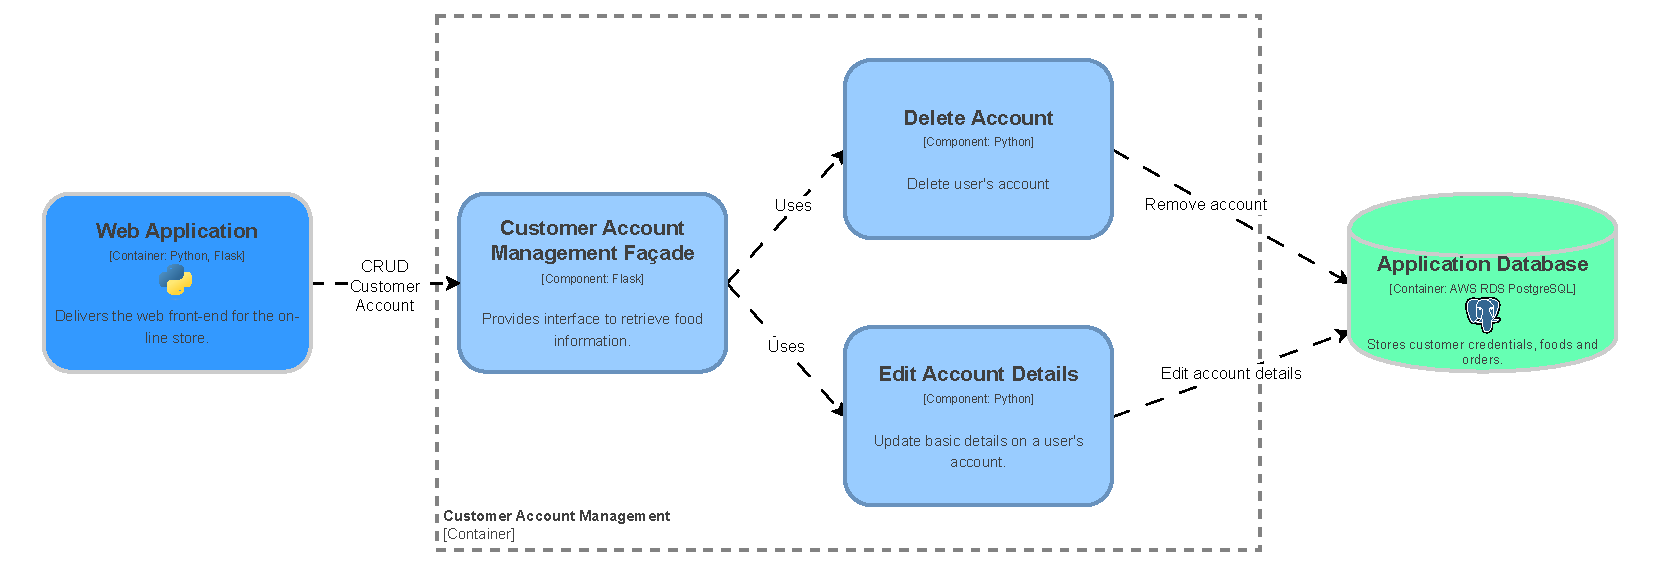
\includegraphics[width=1\linewidth]{model//c4//pdf/customer_account_management_drawio.pdf}
    \caption{Customer Account Management Component Diagram}
    \label{fig:customer}
\end{figure}
\begin{figure}
    \centering
    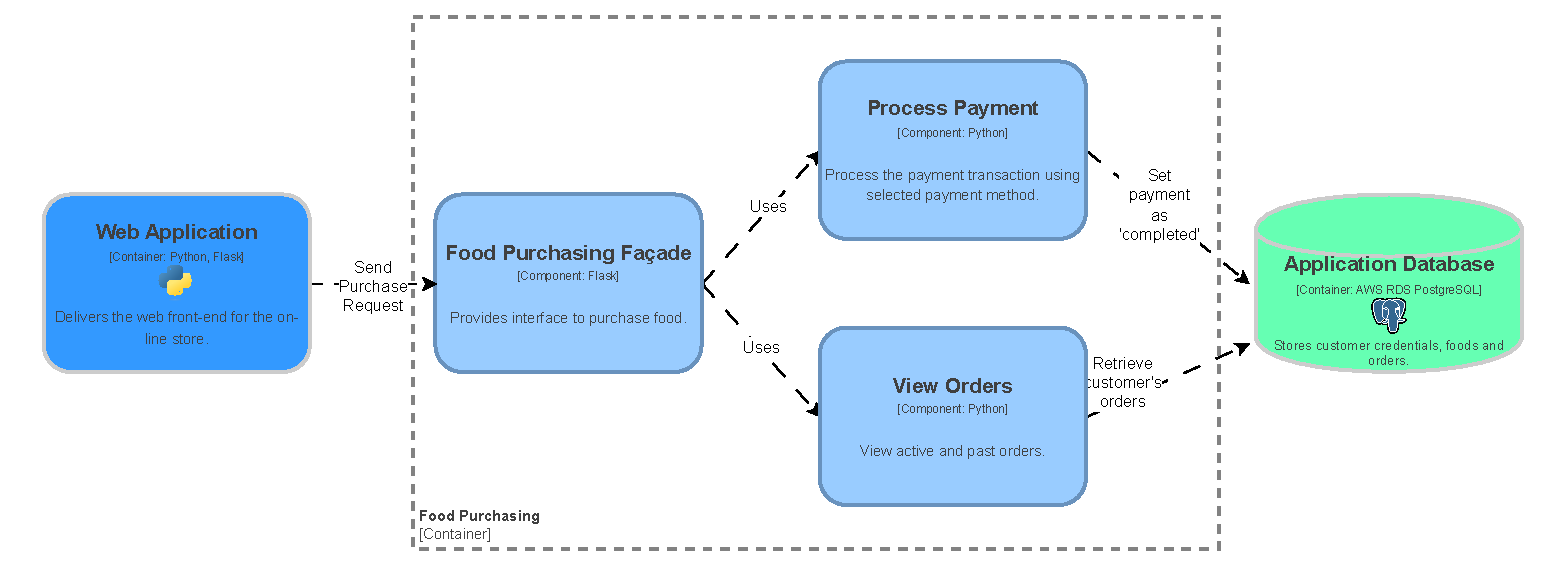
\includegraphics[width=1\linewidth]{model//c4//pdf/food_purchasing_drawio.pdf}
    \caption{Food Purchasing}
    \label{fig:purchase}
\end{figure}
\begin{figure}
    \centering
    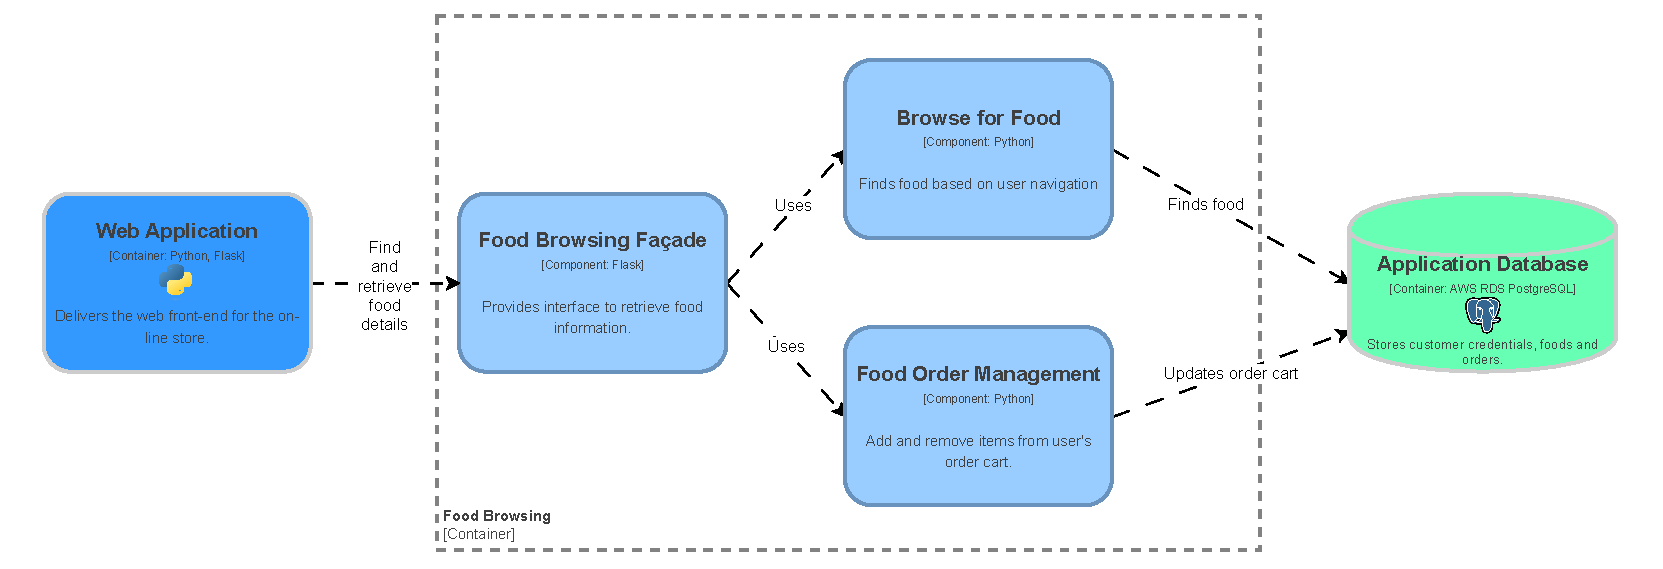
\includegraphics[width=1.0\linewidth]{model//c4//pdf/food_browsing_drawio.pdf}
    \caption{Food Browsing Component Diagram}
    \label{fig:browse}
\end{figure}

\begin{figure}
    \centering
    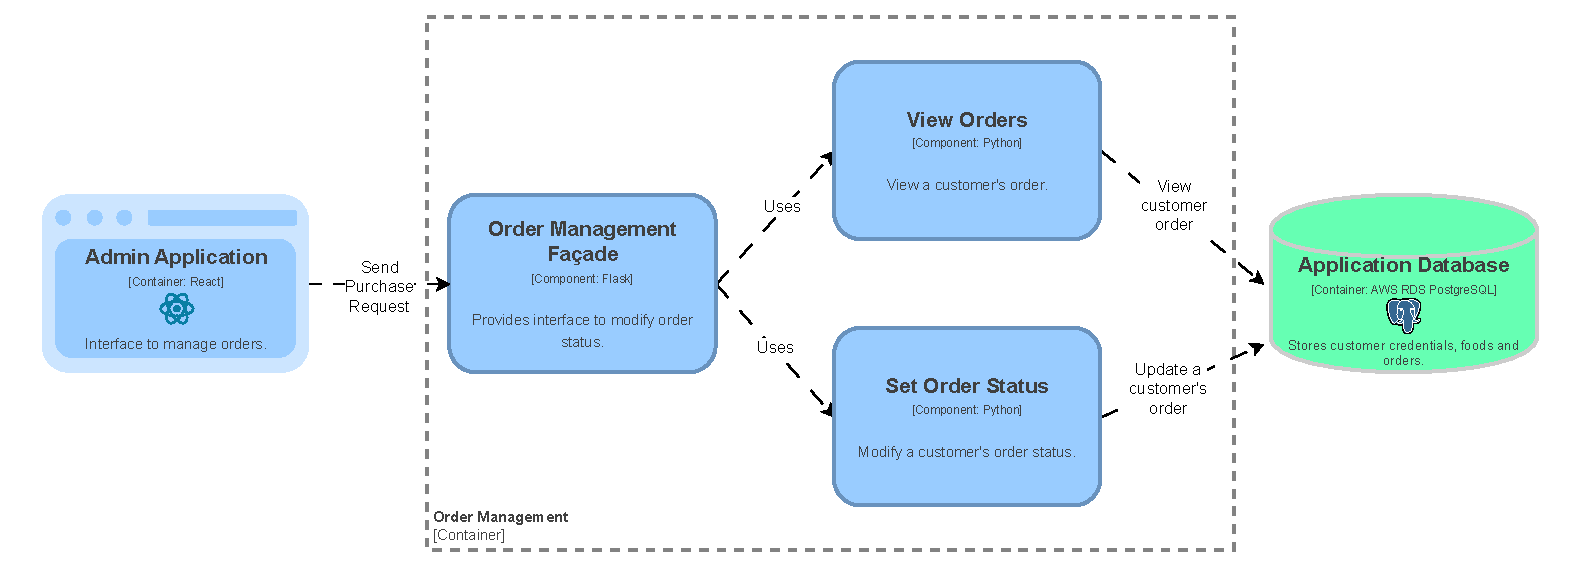
\includegraphics[width=1.0\linewidth]{model//c4//pdf/order_management_drawio.pdf}
    \caption{Order Management Component Diagram}
    \label{fig:orders}
\end{figure}
\restoregeometry






\section{Trade-Offs}
Describe and justify the trade-offs made in designing the architecture.

\subsubsection*{Tradeoff 1. Shared Database}
\begin{minipage}{\dimexpr\textwidth-0.25cm}
\textbf{Problem?} If one service changes its persistent data, then all services that share that data must be changed, as well as the tables storing the data in db
\hfill \break \textbf{Alternative?} Separate database - offers greater flexibility for scaling (in the face of database performance bottlenecks)
\hfill \break \textbf{Justification?}
\begin{itemize}
    \item Some services don't have enough unique data to make it worth creating a separate database for just the service e.g., Customer Account management only needs to validate username and password fields.
    \item The most unique data fields in a service is 4 in the menu-items table (see \ref{fig:db})
    \item For the purposes and scale of this app, it was decided a shared database approach would suffice
    \item Decision made in the interest of reliability, where data integrity and consistency is preserved
    \item There is no need to exchange stored data between services, so API is simplified
    \item An advantage is transaction management - no need to span the transactions over the services
    \item Drawback? Shared database will increase data coupling and lower testability
\end{itemize}
\end{minipage}
\begin{figure}
    \centering
    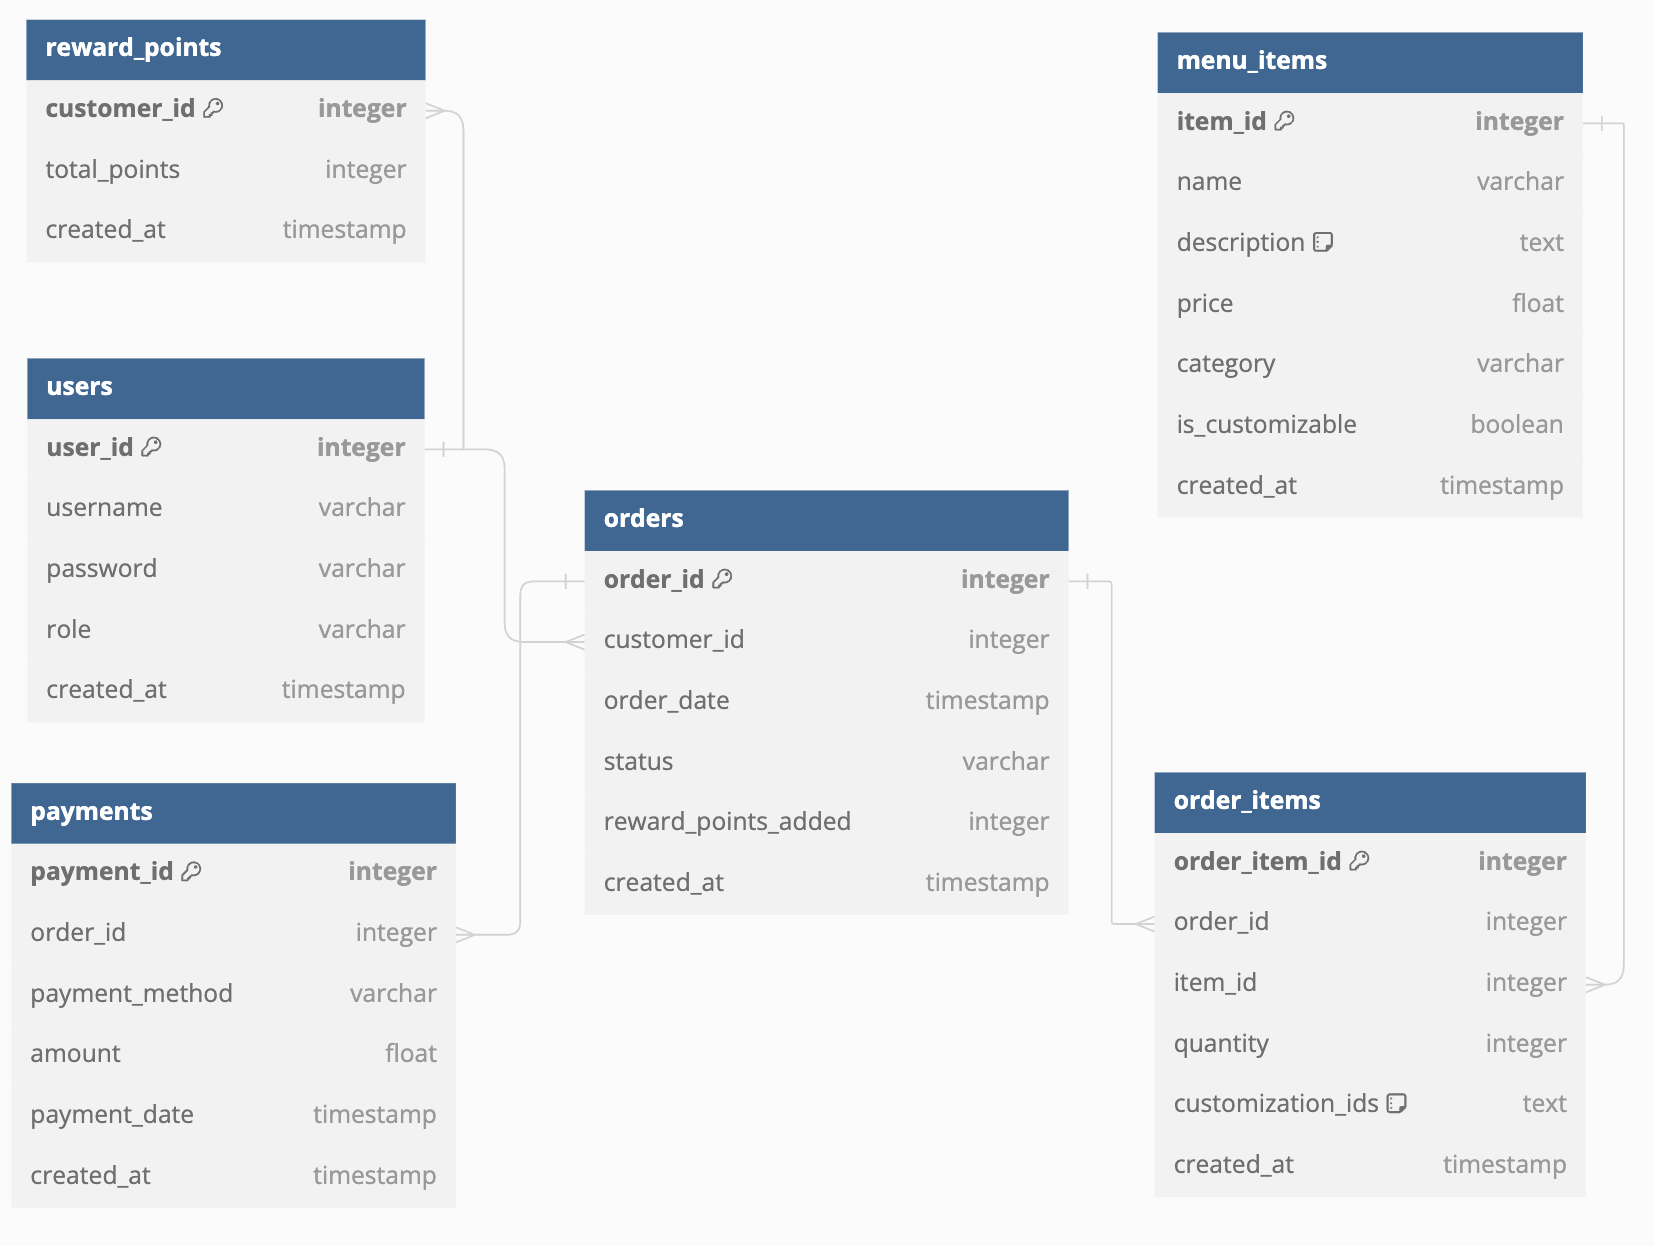
\includegraphics[width=0.75\linewidth]{model/db_diagram.png}
    \caption{Database Design Draft}
    \label{fig:db}
\end{figure}

\section{Critique}
\subsection{Backend Testing Report}

The backend architecture of our food ordering system has been thoroughly tested to ensure it meets the required functionality and quality attributes. The tests included performance tests, functional tests, and stress tests, with particular focus on critical API endpoints. Below are the detailed results of these tests:

\subsubsection*{User Sign-Up and Deletion}

\begin{itemize}
  \item Total Requests: 7116
  \item Successful Requests: 100.00\%
  \item Average HTTP Request Duration: 10.42ms
  \item HTTP Request Failure Rate: 0.00\%
\end{itemize}

These results demonstrate that the user sign-up and deletion functionality is robust, with all requests completing successfully within an average duration of 10.42 milliseconds. This indicates that the system handles these operations efficiently and reliably.

\subsubsection*{Get User Info}

\begin{itemize}
  \item Total Requests: 3605
  \item Successful Requests: 100.00\%
  \item Average HTTP Request Duration: 6.62ms
  \item HTTP Request Failure Rate: 0.00\%
\end{itemize}

The get user info endpoint also performed exceptionally well, with all requests being successful and an average response time of 6.62 milliseconds. This ensures that user information retrieval is quick and dependable.

\subsubsection*{Create Menu Item}

\begin{itemize}
  \item Total Requests: 3606
  \item Successful Requests: 100.00\%
  \item Average HTTP Request Duration: 7.34ms
  \item HTTP Request Failure Rate: 0.00\%
\end{itemize}

Creating menu items showed consistent performance with a 100\% success rate and an average request duration of 7.34 milliseconds. This supports the system's ability to manage menu items efficiently.

\subsubsection*{Get Menu Items}

\begin{itemize}
  \item Total Requests: 1260
  \item Successful Requests: 78.05\%
  \item Average HTTP Request Duration: 1.89s
  \item HTTP Request Failure Rate: 0.00\%
\end{itemize}

The get menu items endpoint, while successful in 78.05\% of cases, had a notably higher average request duration of 1.89 seconds. This suggests a potential bottleneck or inefficiency in retrieving menu data, which may need further optimization to improve user experience.

\subsubsection*{Create Order}
\begin{itemize}
  \item Total Requests: 3584
  \item Successful Requests: 100.00\%
  \item Average HTTP Request Duration: 13.4ms
  \item HTTP Request Failure Rate: 0.00\%
\end{itemize}

Creating orders was also highly efficient, with a 100\% success rate and an average request duration of 13.4 milliseconds. This indicates that the system is capable of handling order creation swiftly and reliably.

\subsection{Architecture Suitability}
The architecture of our system has shown to be well-suited for delivering the required functionality and quality attributes. The following points summarize how the architecture supports key quality attributes:

\subsubsection*{Functionality}
The test results indicate that the system reliably handles user-related operations, menu item management, and order processing. The high success rates and low request durations for most endpoints confirm the functionality is delivered effectively.

\subsubsection*{Performance}
Performance metrics such as average request durations and success rates indicate that the system performs well under the tested conditions. The only area of concern is the get menu items endpoint, which may require optimization.

\subsubsection*{Scalability}
The architecture supports scalability, as evidenced by the system's ability to handle thousands of requests with low failure rates. However, further testing under higher loads and varying conditions would provide additional insights into its scalability.

\subsubsection*{Reliability}
With 100\% success rates in most critical operations, the system demonstrates high reliability. This is crucial for maintaining user trust and ensuring consistent service availability.

\section{Evaluation}
Summarise testing results and justify how well the software achieves its quality attributes.
\section{Reflection}
\subsubsection*{General Reflections on Project}

There were internal decisions within the team that shaped the project delivery. For one, the team underestimated the implementation of a service-based architecture. There were aspects of the implementation that made the process more difficult than anticipated, this included API abstraction and independent services. A better estimation would have led the team to more accurately gauge the project timeline. It also would have helped to implement the missed features discussed below. One decision that proved to be advantageous was opting for Python Flask and not AWS Lambda. AWS Lambda would have offered benefits such as automatic scalability and minimised operational management. However, the team's experience with AWS Lambda was limited to one member. While all others were comfortable with Python Flask. Given the tight timeline for the project, the team feels this was the right decision to ensure an MVP was delivered on time. 

\subsubsection*{Missed Opportunities}
There were two additional features the team wanted to implement.

\medskip \noindent An API layer for security policies would have established a more secure system. A future iteration of the application would use an external payment provider. To prepare for this, a reverse proxy should have been implemented to hide the internal network structure of the system's architecture. This additional layer of abstraction would have been beneficial to delivering the security principle of least privilege. It would also add the possibility for extensions such as security policies, user access logging or service discovery, in the API layer. Time played a major factor in the decision to omit this security feature. As it stands, the internal network structure would be exposed to a future external service, meaning this could be exploited as a security flaw. 

\medskip \noindent Authentication on the admin page would be beneficial for long term security. This feature ideated by the team. It was not in the proposal. Authentication is important to ensure the user accessing the administrative page is in fact an employee. As it stands, the simple solution for now was to create 2 administrative accounts for the employees to securely access. This will still allow the coffee shop to operate and process orders. However, it would likely prove to be unsustainable in the long run, for a coffee shop attempting to expand operations.


\section{References}
\par \sloppy Coffee School. (2022, July 6). How Many Coffees Can a Barista Make in an Hour? – Coffee School. https://www.coffeeschool.com.au/news/how-many-coffees-can-a-barista-make-in-an-hour
\par Fletcher, M. (2016, October 7). Service-Based Architecture as an Alternative to Microservice Architecture. InfoQ. https://www.infoq.com/news/2016/10/service-based-architecture/
\par Richardson, C. (2019). Microservices Pattern: Microservice Architecture pattern. Microservices.Io. Retrieved May 28, 2024, from http://microservices.io/patterns/microservices.html

\footnote{Footnote}




\end{document}
